\begin{figure}[H]	
  \centering
    \resizebox{\linewidth}{!}{\tikzset{font=\Huge}\documentclass{standalone}
\usepackage{tikz}
\usepackage{aeguill}
\begin{document}
% generated by Plantuml 1.2018.12      
\definecolor{plantucolor0000}{RGB}{255,255,255}
\definecolor{plantucolor0001}{RGB}{0,0,0}
\definecolor{plantucolor0002}{RGB}{254,254,206}
\definecolor{plantucolor0003}{RGB}{168,0,54}
\definecolor{plantucolor0004}{RGB}{169,220,223}
\definecolor{plantucolor0005}{RGB}{132,190,132}
\definecolor{plantucolor0006}{RGB}{3,128,72}
\definecolor{plantucolor0007}{RGB}{173,209,178}
\definecolor{plantucolor0008}{RGB}{251,251,119}
\begin{tikzpicture}[yscale=-1
,pstyle0/.style={color=black,fill=white,line width=1.5pt}
,pstyle1/.style={color=black,line width=1.5pt}
,pstyle2/.style={color=plantucolor0003,fill=plantucolor0002,line width=1.5pt}
,pstyle3/.style={color=plantucolor0003,fill=plantucolor0004,line width=1.0pt}
,pstyle4/.style={color=plantucolor0003,line width=1.5pt}
,pstyle5/.style={color=plantucolor0006,fill=plantucolor0005,line width=1.0pt}
,pstyle6/.style={color=plantucolor0003,fill=plantucolor0007,line width=1.0pt}
,pstyle7/.style={color=plantucolor0003,fill=plantucolor0008,line width=1.0pt}
,pstyle8/.style={color=plantucolor0003,line width=1.0pt}
,pstyle9/.style={color=plantucolor0003,fill=plantucolor0003,line width=1.0pt}
,pstyle10/.style={color=black,fill=black,line width=1.0pt}
]
\draw[pstyle0] (294.5pt,16pt) -- (405.3889pt,16pt) -- (412.3889pt,38.4473pt) -- (686.5pt,38.4473pt) -- (686.5pt,125pt) -- (294.5pt,125pt) -- (294.5pt,16pt) -- cycle;
\draw[pstyle1] (294.5pt,38.4473pt) -- (412.3889pt,38.4473pt);
\node at (298.5pt,18pt)[below right,color=black]{\textbf{Framework}};
\draw[pstyle0] (287.5pt,156pt) -- (454.1725pt,156pt) -- (461.1725pt,178.4473pt) -- (743.5pt,178.4473pt) -- (743.5pt,265pt) -- (287.5pt,265pt) -- (287.5pt,156pt) -- cycle;
\draw[pstyle1] (287.5pt,178.4473pt) -- (461.1725pt,178.4473pt);
\node at (291.5pt,158pt)[below right,color=black]{\textbf{ConcreteExample}};
\draw[pstyle2] (302.5pt,43pt) rectangle (484.2285pt,116.6094pt);
\draw[pstyle3] (362.2759pt,59pt) ellipse (11pt and 11pt);
\node at (362.2759pt,59pt)[]{\textbf{\Large A}};
\node at (382.7759pt,52.0156pt)[below right,color=black]{\textit{Creator}};
\draw[pstyle4] (303.5pt,75pt) -- (483.2285pt,75pt);
\draw[pstyle4] (303.5pt,83pt) -- (483.2285pt,83pt);
\draw[pstyle5] (313.5pt,94.9023pt) ellipse (3pt and 3pt);
\node at (322.5pt,87pt)[below right,color=black]{anOperation()};
\draw[pstyle5] (313.5pt,107.707pt) ellipse (3pt and 3pt);
\node at (322.5pt,99.8047pt)[below right,color=black]{\textit{factoryMethod():Product}};
\draw[pstyle2] (591pt,43pt) rectangle (677.8816pt,116.6094pt);
\draw[pstyle3] (606pt,59pt) ellipse (11pt and 11pt);
\node at (606pt,59pt)[]{\textbf{\Large A}};
\node at (620pt,52.0156pt)[below right,color=black]{\textit{Product}};
\draw[pstyle4] (592pt,75pt) -- (676.8816pt,75pt);
\draw[pstyle4] (592pt,83pt) -- (676.8816pt,83pt);
\node at (597pt,87pt)[below right,color=black]{\textit{method1()}};
\node at (597pt,99.8047pt)[below right,color=black]{\textit{method2()}};
\draw[pstyle2] (296pt,189.5pt) rectangle (474.5266pt,250.3047pt);
\draw[pstyle6] (323.1345pt,205.5pt) ellipse (11pt and 11pt);
\node at (323.1345pt,205.5pt)[]{\textbf{\Large C}};
\node at (339.831pt,198.5156pt)[below right,color=black]{ConcreteCreator};
\draw[pstyle4] (297pt,221.5pt) -- (473.5266pt,221.5pt);
\draw[pstyle4] (297pt,229.5pt) -- (473.5266pt,229.5pt);
\draw[pstyle5] (307pt,241.4023pt) ellipse (3pt and 3pt);
\node at (316pt,233.5pt)[below right,color=black]{factoryMethod():Product};
\draw[pstyle2] (582pt,183pt) rectangle (734.6667pt,256.6094pt);
\draw[pstyle6] (597pt,199pt) ellipse (11pt and 11pt);
\node at (597pt,199pt)[]{\textbf{\Large C}};
\node at (611pt,192.0156pt)[below right,color=black]{ConcreteProduct};
\draw[pstyle4] (583pt,215pt) -- (733.6667pt,215pt);
\draw[pstyle4] (583pt,223pt) -- (733.6667pt,223pt);
\node at (588pt,227pt)[below right,color=black]{method1()};
\node at (588pt,239.8047pt)[below right,color=black]{method2()};
\draw[pstyle7] (6pt,202.5pt) -- (6pt,227.6328pt) -- (260.6589pt,227.6328pt) -- (260.6589pt,220.5pt) -- (300pt,239.9023pt) -- (260.6589pt,212.5pt) -- (260.6589pt,212.5pt) -- (250.6589pt,202.5pt) -- (6pt,202.5pt);
\draw[pstyle7] (250.6589pt,202.5pt) -- (250.6589pt,212.5pt) -- (260.6589pt,212.5pt) -- (250.6589pt,202.5pt);
\node at (12pt,207.5pt)[below right,color=black]{return new ConcreteProduct();};
\draw[pstyle8] (484.6118pt,80pt) ..controls (518.8691pt,80pt) and (556.5013pt,80pt) .. (585.4886pt,80pt);
\draw[pstyle9] (590.7978pt,80pt) -- (581.7978pt,76pt) -- (585.7978pt,80pt) -- (581.7978pt,84pt) -- (590.7978pt,80pt) -- cycle;
\node at (502.75pt,61pt)[below right,color=black]{Creates};
\draw[pstyle10] (563.2439pt,67.0664pt) -- (569.2439pt,70.0664pt) -- (563.2439pt,73.0664pt) -- (563.2439pt,67.0664pt) -- cycle;
\draw[pstyle8] (475.2685pt,220pt) ..controls (508.0172pt,220pt) and (544.8471pt,220pt) .. (576.8514pt,220pt);
\draw[pstyle9] (581.9451pt,220pt) -- (572.9451pt,216pt) -- (576.9451pt,220pt) -- (572.9451pt,224pt) -- (581.9451pt,220pt) -- cycle;
\node at (493.5pt,201pt)[below right,color=black]{Creates};
\draw[pstyle10] (553.9939pt,207.0664pt) -- (559.9939pt,210.0664pt) -- (553.9939pt,213.0664pt) -- (553.9939pt,207.0664pt) -- cycle;
\draw[pstyle8] (390.2284pt,137.2538pt) ..controls (389.2102pt,155.0722pt) and (388.1268pt,174.0309pt) .. (387.2543pt,189.2994pt);
\draw[pstyle8] (383.2475pt,136.7179pt) -- (391.3772pt,117.1499pt) -- (397.2247pt,137.5167pt) -- (383.2475pt,136.7179pt) -- cycle;
\draw[pstyle8] (644.2673pt,136.9759pt) ..controls (646.9079pt,152.3797pt) and (649.6981pt,168.6556pt) .. (652.1017pt,182.6765pt);
\draw[pstyle8] (637.3486pt,138.0451pt) -- (640.8685pt,117.1499pt) -- (651.1473pt,135.6795pt) -- (637.3486pt,138.0451pt) -- cycle;
\end{tikzpicture}
\end{document}
}
\end{figure}
\begin{intentbox}[Intent]\\
  \begin{itemizenosep}
    \item
    Making program code independent of concrete classes:
    \item 
    a class can't anticipate the class of objects it must create
    \item
    a class wants its subclasses to specify the objects it creates
\end{itemizenosep}
\imp{Thus}: creating objects by calling a factory method—either specified in an interface and implemented by child classes, or implemented in a base class and optionally overridden by derived classes—rather than by calling a constructor.
\end{intentbox}
{\centering
\begin{minipage}[t]{0.5\columnwidth}
  \begin{codeboxNl}[Bad (statically typed)]{java}
        Interf_X ref = new X();
  \end{codeboxNl}
\end{minipage}
\begin{minipage}[t]{0.45\columnwidth}
  \begin{codeboxNl}[factoryMethod]{java}
        InterfX ref = cCreat.getX();
  \end{codeboxNl}
\end{minipage}}
\begin{figure}[H]
  \centering
  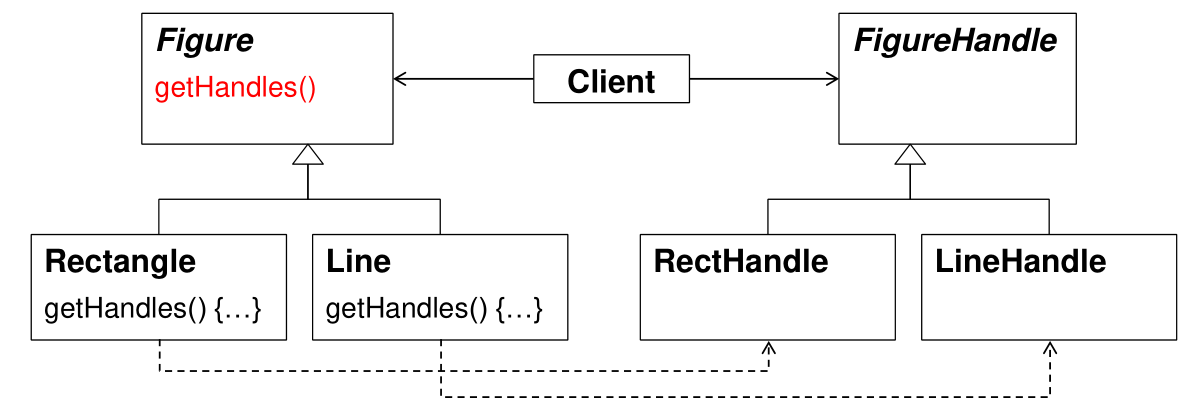
\includegraphics[width=1.0\columnwidth]{figures/factoryMethodHandles.png}
  \caption{}
  \label{fig:}
\end{figure}
\begin{defnbox}\nospacing
  \begin{defn}[GOF Definition]\label{defn:}
    Define an interface for creating an object, but let subclasses decide which class to instantiate. Factory Method lets a class defer instantiation to subclasses. 
  \end{defn}
\end{defnbox}
\begin{notebox}[Note]\nospacing
  People often use Factory Method as the standard way to create objects; but it isn't necessary if: the class that's instantiated never changes.
\end{notebox}
\begin{notebox}[Note]\nospacing
  The Factory Method pattern has commonly been misunderstood to mean any method whose sole purpose is to construct an object and return this created object. In most cases, this translates to a static method that abstracts the construction process of an object
\end{notebox}
\begin{partbox}[Participants]
  \begin{itemizenosep}
    \item \imp{Abstrac/Interface Product}: specifies type of product to be
  created e.g.\ HandleType
    \item \imp{Abstrac/Interface Creator}: Object that will instantiate the
  product may be
  \begin{itemize}
      \item an \javainline{interface} which includes one or more Factory
    Methods, as well as any number of other methods.
      \item an \javainline{abstract class}
    with defined methods or even a default implementation of the Factory Method that returns a default instance of Product. 
  \end{itemize}
    \item \imp{Concrete Creator}: creator class ($\neq$ factory)s that uses
    factory method \& returns different \javainline{ConcreteProduct} instances
    (that all implement the Product interface) depending on the the concrete
    creator. 
  \end{itemizenosep}
\end{partbox}
\begin{sectionbox}[Implementation]\nospacing
  \begin{itemizenosep}
      \item \imp{In a static method}: simplified version of factoryMethod
    (pattern):
    where the Creator hierarchy is reduced to a single class and the factory
    method is reduced to a single static method (rather than a method that is
    overridden for each of the possible products).\\
    The use of this \javainline{static method} allows for a single point of
    entry into a library. We use the class in order to obtain a conrete object.
    \begin{mintlinebox}{java}
      public class XmlHandlerFactory {
        public static XmlHandler createHandler() {
          return new XmlPrintHandler();
        }
      }
      |\optldots|
      XmlHandler handler = XmlHandlerFactory.createHandler();
    \end{mintlinebox}
      \item \imp{Sub classes}: as discussed above
      \item \imp{In an separate object} = \rdb{Abstract Factory pattern}
  \end{itemizenosep}
\end{sectionbox}
\begin{notebox}[Note: static approach]\nospacing
  assumes that the \javainline{XmlHandler} creator has enough knowledge to know
  which handler implementation is appropriate.
\end{notebox}
\begin{notebox}[Difference Abstrac Factroy]\nospacing
  Factory Method is similar to Abstract Factory but without the emphasis on families.
\end{notebox}
\begin{codeboxNl}[Product Interface]{java}
public interface EncryptionAlgorithm {
  public String encrypt(String plaintext);
}
\end{codeboxNl}
\begin{codeboxNl}[Concrete Product]{java}
public class Sha512EncryptionAlgorithm implements EncryptionAlgorithm {
  @Override
  public String encrypt(String plaintext) {
      return DigestUtils.sha512Hex(plaintext);
  }
}
\end{codeboxNl}
\begin{codeboxNl}[Abstract Creator]{java}
 public abstract class Encryptor {
  public void writeToDisk(String plaintext, String filename) {
      EncryptionAlgorithm encryptionAlgorithm = getEncryptionAlgorithm();
      String cyphertext = encryptionAlgorithm.encrypt(plaintext);
      |\optldots|
  }
  public abstract EncryptionAlgorithm getEncryptionAlgorithm();
} 
\end{codeboxNl}
\begin{codeboxNl}[ConcreteCreator]{java}
  public class Sha256Encryptor extends Encryptor {
    @Override
    public EncryptionAlgorithm getEncryptionAlgorithm() {
        return new Sha256CEncryptionAlgorithm();
    }
}
\end{codeboxNl}
\begin{sectionbox}[Implementation Issues]\nospacing
  \begin{itemizenosep}
      \item static factory implementations method cannot be overridden (as the
    method is static) $\Rightarrow$ can be compared to a \javainline{final factory method} \item Factory methods my be parameterized to describe the product it
    creates:
    \begin{mintlinebox}{java}
      Product createProduct(ProductID id)
    \end{mintlinebox}
    \item Factory Method in abstract base class may provide default return type.
  \end{itemizenosep}
\end{sectionbox}
%%% Local Variables:
%%% mode: latex
%%% TeX-master: "../formulary"
%%% End:
